\section{Análisis de datos}
Para cada host destino se ha monitoreado la ruta durante un tiempo considerable.
De esta manera se ha buscado que los datos se estabilicen y sean lo más certero posible.\\

A continuación detallamos la información obtenida en las mediciones. Es importante aclarar que en las tablas de monitoreo la información de Ubicación
fue obtenida de la herramienta $http://www.plopip.com/$. Cómo hemos hallado inconsistencias, dicha ubicación podría ser modificada en las conclusiones finales.

\subsection{Universidad París Descartes - Francia}
Presentamos en la siguiente tabla los resultados obtenidos del último monitoreo.

\bigskip

\begin{tabular}{ | l | c | c | c | c |}
 \hline                 
   Hop & IP &  RTT promedio (s)  & deltaRTT promedio & Ubicación\\
 \hline 
   1 & 192.168.0.1 & 0,006502 & 0,006502 & Argentina - Buenos Aires\\ 
 \hline 
   2 & 200.89.164.189 & 0,025426 & 0,018924 & Argentina - Buenos Aires\\ 
  \hline 
   3 & 200.89.165.5 & 0,022739 & 0 & Argentina - Buenos Aires\\ 
  \hline 
   4 & 200.89.165.250 & 0,023967 & 0,001227 & Argentina - Buenos Aires\\ 
  \hline 
   5 & 206.165.31.213 & 0,023886 & 0 & Estados Unidos\\ 
  \hline 
   6 & 67.16.139.18 & 0.153896 & 0,130009 & Estados Unidos - Manhattan\\ 
  \hline 
   7 & 213.248.76.189 & 0,147402 & 0 & Europa (Telia Network Services)\\ 
  \hline 
   8 & 62.115.143.64 & 0,173705 & 0,026303 & Europa (Telia Network Services UK)\\ 
  \hline 
   9 & 213.155.130.86 & 0,174316 & 0,000610 & Europa (Telia Network Services UK)\\ 
  \hline 
   10 & 80.239.132.130 & 0,183801 & 0,009485 & Alemania (Telia AB/Telia Int. Carrier)\\ 
  \hline 
   11 & 195.2.30.46 & 0,249497 & 0,065696 & Europa\\ 
  \hline 
   12 & 195.2.28.154 & 0,244204 & 0 & Europa\\ 
  \hline 
   13 & 195.2.10.145 & 0,243621 & 0 & Europa\\ 
  \hline 
   14 & 195.10.54.66 & 0,269441 & 0,025820 & Francia (Dyson Ltd)\\ 
  \hline 
   15 & 193.51.177.25 & 0,271685 & 0,002243 & Francia - Paris\\ 
  \hline 
   16 & 193.51.177.116 & 0,258662 & 0 & Francia - Paris\\ 
  \hline 
   17 & 193.51.181.101 & 0,258660 & 0 & Francia - Paris\\
  \hline 
   18 & 195.221.127.166 & 0,269296 & 0,010635 & Francia - Paris\\
  \hline 
   19 & 193.51.86.16 & 0,256802 & 0 & Francia\\
  \hline 
   20 & 193.51.181.101 & 0,258082 & 0,001279 & Francia\\
  \hline 
   21 & 193.51.181.101 & 0,254919 & 0 & Francia\\
  \hline 
   22 & 193.51.181.101 & 0,255926 & 0,001007 & Francia\\
  \hline 
   23 & 193.51.181.101 & 0,254769 & 0 & Francia\\
  \hline 
   24 & 193.51.181.101 & 0,256566 & 0,001797 & Francia\\    
 \hline 
\end{tabular}

\bigskip

Con estos datos hemos obtenido que los $\Delta$ $RTT$ siguen una distribución normal con una probabilidad del 99,5$\%$ ($\alpha$ $=$ 0,005).
Se ha realizado el test de $Grubbs$ y nos ha devuelto que los $outliers$ se encuentran en los saltos 6 y 11.\\

A continuación mostramos que ocurre con los $RTT$ promedio de cada salto y con los $zScore$ promedio de cada salto:

\begin{figure}[H]
\centering
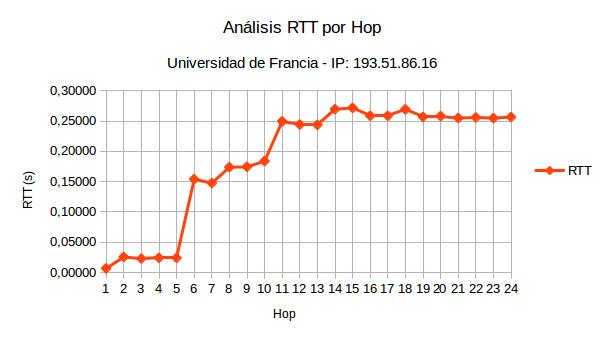
\includegraphics[width=1\textwidth]{graficos/rTT_Francia.jpg}
\caption{RTT promedio por hop - Universidad de Francia}
\label{francia_rtt}
\end{figure}

\begin{figure}[H]
\centering
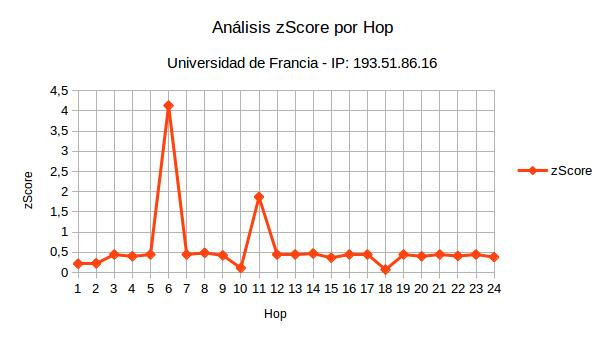
\includegraphics[width=1\textwidth]{graficos/zScore_Francia.jpg}
\caption{zScore promedio por hop - Universidad de Francia}
\label{francia_zs}
\end{figure}

En ambos gráficos se puede apreciar como en los saltos 6 y 11 (los que nos habían dado como $outliers$ en el test de $Grubbs$) hay un cambio abrupto 
en la distribución de los datos. En el gráfico de $RTT$ podemos notar cómo sube de golpe el $RTT$ promedio. En el otro gráfico podremos observar cómo 
se forman picos en estos saltos.\\

Nos ha llamado la atención que figuren dos $outliers$ cuando el enlace submarino debería ser solamente uno para ir hacia Francia. 
Verificando las ubicaciones de los host intermedios notamos que el primer $outlier$ corresponde a un host que se encuentra en Estados Unidos 
(el cual nosotros desde Argentina estamos a más de 8000 kilómetros). El salto 5, según nos indica la herramienta de geolocalización, se encontraría
en Estados Unidos pero no creemos que sea cierto dado que el $RTT$ es muy similar a los hosts ubicados en Argentina.\\

El segundo $outlier$ detectado corresponde al salto 11 donde ya nos ubicamos en un host europeo. Aquí claramente ya hemos atravesado un 
enlace submarino desde Estados Unidos hacia Europa. También nos ha llamado la atención al localizar los hosts anteriores del salto 11: los hemos 
localizado en Europa. Sin embargo no tienen un cambio de $RTT$ significativo por lo que estimamos que se encuentran en Estados Unidos. Los saltos 7, 8, 9 y 10
corresponden a hosts de la empresa de telecomunicaciones Telia y estimamos que debe contratar servicios en Estados Unidos. Por este motivo no notamos 
en los $RTT$ cambios abruptos ni picos en los $zScore$ obtenidos.\\

Para los demás saltos hemos notado que los $\Delta$ $RTT$ son similares y los host debe estar equidistantes hasta llegar al host destino dado que no 
hemos observado valores atípicos.\\

A continuación hemos trazado en un mapa la ruta de nuestro host hasta el host destino ubicado en Francia:
%\begin{figure}[H]
%\centering
%\includegraphics[width=1\textwidth]{graficos/mapa_Francia.jpg}
%\caption{Ruta en Internet - Universidad de Francia}
%\label{francia_zs}
%\end{figure}



 \subsection{Universidad de Mosku - Rusia}

Como tercer caso de estudio, tomamos el servidor de la universidad de mosku (www.msu.ru). El traceroute obtenido para esta universidad es el siguiente:

\bigskip

\begin{tabular}{| l | c | c | c | c |}
 \hline 
Hop & IP &  RTT promedio (s)  & deltaRTT promedio & Ubicación\\
\hline 
1  &  192.168.0.1  &  0.00328697348541    &  0.00328697348541 & Argentina\\
\hline 
2  &  200.89.164.165  &  0.0182673031429    &  0.0149803296575 & Argentina\\
\hline 
3  &  200.89.165.130  &  0.018018808005    &  0 & Argentina\\
\hline 
4  &  200.89.165.222  &  0.023129620642   &  0.00511081263704 & Argentina\\
\hline 
5  &  206.165.31.213  &  0.0159362801966    &  0 & United States\\ 
\hline 
6  &  67.17.75.66  &  0.153266360362    &  0.137330080166 &  United States\\
\hline 
7  &  4.68.111.121  &  0.144784176125    &  0 & United States\\ 
\hline 
8  &  4.69.158.253  &  0.267091494686    &  0.122307318561 &  United States\\
\hline 
9  &  4.69.158.253  &  0.266443899045    &  0 & United States\\
\hline 
10  &  213.242.110.198  &  0.313186002227    &  0.0467421031829 & United Kingdom\\
\hline 
11  &  194.85.40.229  &  0.313147967716    &  0 & Russian Federation\\
\hline 
12  &  194.190.254.118  &  0.295875315396    &  0 & Russian Federation\\
\hline 
13  &  93.180.0.172  &  0.310500500249   &  0.0146251848526 & Moscow City Russian Federation\\
\hline 
14  &  188.44.33.30  &  0.293746012562    &  0 & Moscow City\\
\hline 
15  &  188.44.50.103  &  0.286035416261   &  0 & Moscow City\\
\hline 
\end{tabular}

De manera preliminar puede verse que la diferencia temporal entre los diferentes hops permanece en el orden de los $10^-3$ segundos, 
habiendo tan solo dos casos en que esto no sucede. Primero en el salto $6$ y luego en el salto $8$ que se encuentran en el orden de los $10^-1$ 
segundos.

A continuación se muestra el grafico de los RTT en cada hop, donde puede verse de manera visual que los saltos temporales mas abruptos se dan en 
el 6 y en el 8:

\bigskip

\begin{figure}[H]
\centering
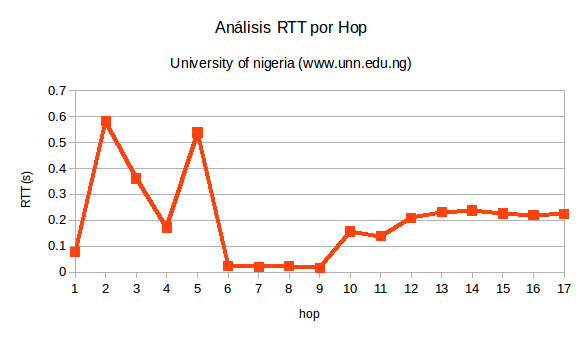
\includegraphics[width=1\textwidth]{graficos/zScore_rus.png}
\caption{zScore promedio por hop - Universidad de Mosku}
\label{Rus_zs}
\end{figure}

En este momento realizamos el test de hipotesis para ver si podemos aproximar los reslutados de los delta rtt a una distribución normal. 
El test de hipotesis que podemos aceptar la hipotesis con una confianza de $0.995$

Por lo tanto calculamos los zScore donde podremos apreciar cuan alejados estan los valores de la media y los graficamos:

\begin{figure}[H]
\centering
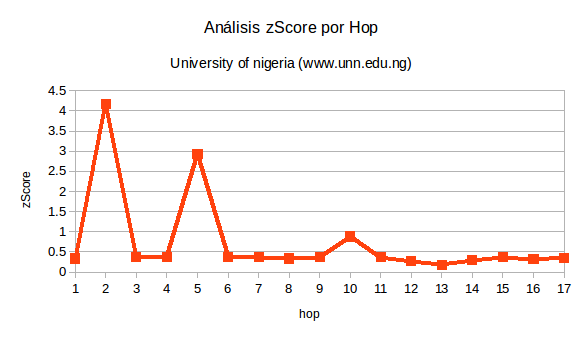
\includegraphics[width=1\textwidth]{graficos/RTT_rus.png}
\caption{RTT promedio por hop - Universidad de Mosku}
\label{Rus_rtt}
\end{figure}

Aqui tambien puede verse que los valores 6 y 8 son los mas patologicos y por lo tanto, los mejores candidatos a ser enlaces submarinos.

Finalmente utilizando el test de grubbs, obtenemos que efectivamente estos valores son outliers dentro de esta distribución normal, y por lo tanto, los saltos que mas probablemente correspondan a saltos submarinos.

Aun asi resulta extraño ver que tanto en el hop 6 como en el 8 las ips dicen estar asignadas a estados unidos. Esto podría deberse a que aunque las ips esten asignadas a estados unidos, el lugar fisico donde se encuentren sea otro.

Utilizando la herramienta http://www.infobyip.com/ pudimos observar algunos de los nombres de los hosts por los cuales hicimos el traceroute.

De esto conseguimos la siguiente tabla:

\begin{tabular}{| l | c | c }
\hline 
hop & IP & Host name\\
\hline 
5  &  206.165.31.213  &  xe-8-3-0.ar3.eze1.gblx.net\\
\hline 
6  &  67.17.75.66  &   po3-20G.ar3.MIA2.gblx.net\\
\hline 
7  &  4.68.111.121  & ae5.edge2.miami2.level3.net\\
\hline 
8  &  4.69.158.253  & ae-114-3504.bar1.Stockholm1.Level3.net\\
\end{tabular}

Tomando como hipotesis que los nombres de los hosts se correspondan con su hubicación geografica, entonces nuestros resultados sobre 
cuales son los saltos submarinos parecerían tener sentido ya que del salto 5 al salto 6 el paquete habría viajado desde argentina hasta miami y 
del salto 7 al salto 8 el paquete pareceria haber viajado de miami a estocolmo.

\subsection{The Hong Kong University of Technology and Science - Hong Kong - IP: 193.51.86.16}

Para esta IP monitoriamos el traceroute hasta el número 90. Presentamos en la siguiente tabla los resultados obtenidos.

\bigskip

\begin{tabular}{ | l | c | c | c | c |}
	\hline
		Hop & IP &  RTT promedio (s)  & deltaRTT promedio & Ubicación\\
 	\hline
		1  &  192.168.0.1  &  0.021503 &  0.021503 & Argentina - Buenos Aires \\
	\hline
		2  &  200.89.166.177  &  0.028651 &  0.007148 & Argentina - Buenos Aires\\
	\hline
		3  &  200.89.165.130  &  0.025739 &  0 & Argentina - Buenos Aires\\
	\hline
		4  &  200.89.165.222  &  0.031074 &  0.005334 & Argentina - Buenos Aires\\
	\hline
		5  &  208.178.195.205  &  0.02794 &  0 & Estados Unidos - Florida \\
	\hline
		6  &  67.17.106.162  &  0.1641088 &  0.136164 & Estados Unidos - Kansas \\
	\hline
		7  &  64.212.107.98  &  0.1607451 &  0 & Estados Unidos - Kansas \\
	\hline
		8  &  129.250.3.172  &  0.1631746 &  0.002429 & Estados Unidos - Colorado \\
	\hline
		9  &  129.250.2.219  &  0.1854111 &  0.022236 & Estados Unidos - Colorado\\
	\hline
		10  &  129.250.7.69  &  0.1903247 &  0.004913 & Estados Unidos - Colorado \\
	\hline
		11  &  129.250.2.177  &  0.307158 &  0.116833 & Estados Unidos - Colorado \\
	\hline
		12  &  129.250.6.144  &  0.313425 &  0.006267 & Estados Unidos - Colorado\\
	\hline
		13  &  129.250.2.222  &  0.366600 &  0.0531743 & Estados Unidos - Colorado\\
	\hline
		14  &  129.250.6.125  &  0.351373 &  0 & Estados Unidos - Colorado \\
	\hline
		15  &  129.250.3.11  &  0.3576226 &  0.006249 & Estados Unidos - Colorado\\
	\hline
		16  &  203.131.246.154 &  0.391269 &  0.0336466 & Hong Kong - Districto Central \\
	\hline
		17  &  115.160.187.110 &  0.387334 &  0 & Hong Kong - Districto Central\\
	\hline
		18  &  202.130.98.102  &  0.373508 &  0 & Hong Kong - Districto Central\\
	\hline
		19  &  203.188.117.130 &  0.380355 &  0.006846 & Hong Kong - Districto Central\\
	\hline
		20  &  202.14.80.153  &  0.378142 &  0 & Hong Kong - Districto Central\\
	\hline
		21  &  143.89.14.2  &  0.380775 &  0.002632 & Hong Kong - Districto Central\\
	\hline
		22  &  143.89.14.2  &  0.382564 &  0.001789 & Hong Kong - Districto Central\\
	\hline
		23  &  143.89.14.2  &  0.383357 &  0.000793 & Hong Kong - Districto Central\\
	\hline
		24  &  143.89.14.2  &  0.384837 &  0.001479 & Hong Kong - Districto Central\\
	\hline
		25  &  143.89.14.2  &  0.384046 &  0 & Hong Kong - Districto Central\\
	\hline
		26  &  143.89.14.2  &  0.385690 &  0.001644 & Hong Kong - Districto Central\\
\hline
\end{tabular}

\bigskip

En base a los resultados obtenidos tomamos los $Delta$ $RTT$ y realizamos un test de normalidad de nivel $alpha$ $0.005$ y podemos concluir que sigue una distribución Normal. \\

Además realizamos el Test de Grubbs para determinar la existencia de outliers, dichos valores representan a los saltos oceánicos, es decir cuando un paquete realiza un salto de un servidor situado en un continente distinto al del salto anterior.\\
El test nos dio $Rechadazo$, como era de esperarse, debido a que realizamos una consulta a una Universidad situada en el continente asiatico. Para sorpresa nuestra, detectamos outliers en los Hop 6 y 11. El número 11 efectivamente es un salto oceanico, ya que pasa de un router situado en $Estados Unidos$ a uno en $Hong Kong$. En cambio el número 6 es un salto desde $Argentina$ a $Estados Unidos$, debido a la distancia entre un router y otro nuestro test lo detecta como un salto oceánico, a pesar de no serlo.\\

Presentamos un mapa que muestra la ubicación geográfica de los saltos\\

\begin{figure}[H]
\centering
\includegraphics[width=1\textwidth]{graficos/mapa_HongKong.jpg}
\caption{Saltos hacia la Universidad de Hong Kong}
\label{hongkong_rtt}
\end{figure}


\begin{figure}[H]
\centering
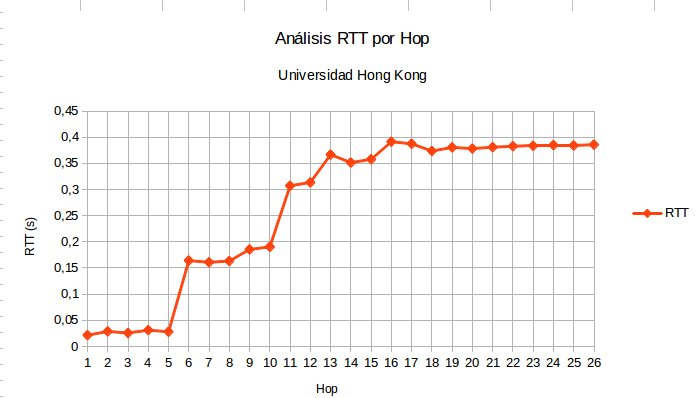
\includegraphics[width=1\textwidth]{graficos/rTT_HongKong.jpg}
\caption{RTT promedio por hop - Universidad de Hong Kong}
\label{hongkong_rtt}
\end{figure}

\begin{figure}[H]
\centering
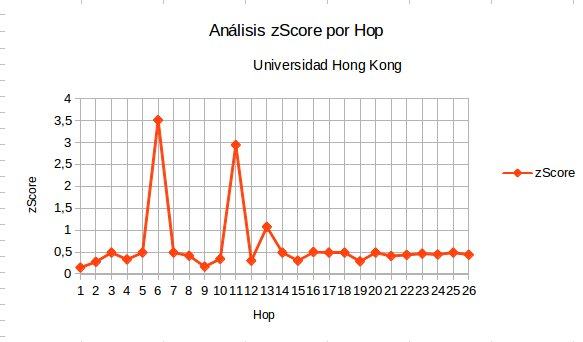
\includegraphics[width=1\textwidth]{graficos/zScore_HongKong.jpg}
\caption{zScore promedio por hop - Universidad de Hong Kong}
\label{hongkong_zs}
\end{figure}


\subsection{Universidad de Sydney - Australia}
Presentamos en la siguiente tabla los resultados obtenidos del último monitoreo.

\bigskip

\begin{tabular}{ | l | c | c | c | c |}
 
  \hline                 
  Hop & IP &  RTT promedio (s)  & deltaRTT promedio & Ubicación\\
  \hline
  1  &  192.168.0.1  &  0.00317819338096  &  0.00317819338096 & Argentina - Buenos Aires\\
  \hline
  2  &  200.89.165.169  &  0.0273115007501  &  0.0241333073691 & Argentina - Buenos Aires\\
  \hline
  3  &  200.89.165.5  &  0.0295196944161  &  0.00220819366606 & Argentina - Buenos Aires\\
  \hline
  4  &  200.89.165.250  &  0.0303499635897  &  0.000830269173572 & Argentina - Buenos Aires\\
  \hline
  5  &  207.136.166.241  &  0.0279953793476  &  0 & Estados Unidos\\
  \hline
  6  &  67.16.139.18  &  0.15700549953  &  0.129010120183 & Estados Unidos - Illinois\\
  \hline
  7  &  64.208.27.102  &  0.151270602879  &  0 & Estados Unidos\\
  \hline
  8  &  129.250.3.172  &  0.15870277662  &  0.00743217374149 & Estados Unidos - Colorado\\
  \hline
  9  &  129.250.2.219  &  0.176934030495  &  0.0182312538749 & Estados Unidos - Colorado\\
  \hline
  10  &  129.250.7.69  &  0.185023287409  &  0.00808925691404 & Estados Unidos - Colorado\\
  \hline
  11  &  129.250.3.123  &  0.185811053765  &  0.000787766356217 & Estados Unidos - Colorado\\
  \hline
  12  &  204.1.253.166  &  0.185876883959  &  6.58301930679e-05 & Estados Unidos - California\\
  \hline
  13  &  202.158.194.172  &  0.3106533885  &  0.124776504542 & Australia - New South Wales\\
  \hline
  14  &  113.197.15.68  &  0.305794251593  &  0 & Australia - New South Wales\\
  \hline
  15  &  113.197.15.66  &  0.331599779819  &  0.0258055282267 & Australia - New South Wales\\
  \hline
  16  &  113.197.15.62  &  0.330528166733  &  0 & Australia - New South Wales\\
  \hline
  17  &  113.197.15.13  &  0.330654288593  &  0.000126121859801 & Australia - New South Wales\\
  \hline
  18  &  138.44.5.47  &  0.337141043261  &  0.00648675466839 & Australia\\
  \hline
  19  &  129.78.5.11  &  0.337009869124  &  0 & Australia - Sydney\\
  \hline
  20  &  129.78.5.11  &  0.337688013127  &  0.000678144003216 & Australia - Sydney\\
  \hline
  21  &  129.78.5.11  &  0.336762147514  &  0 & Australia - Sydney\\
  \hline
  22  &  129.78.5.11  &  0.338513030818  &  0.00175088330319 & Australia - Sydney\\
  \hline
  23  &  129.78.5.11  &  0.336039300028  &  0 & Australia - Sydney\\
  \hline
  24  &  129.78.5.11  &  0.339367595158  &  0.00332829513048 & Australia - Sydney\\
  \hline

\end{tabular}

\bigskip

\begin{figure}[H]
\centering
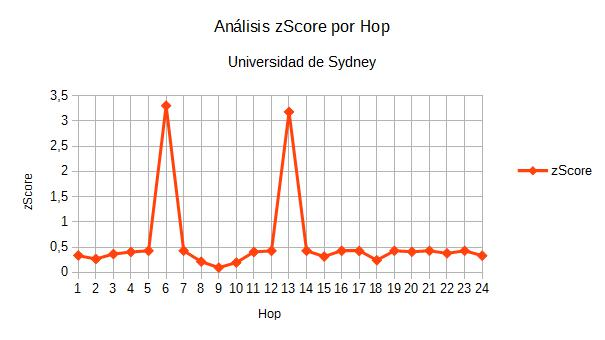
\includegraphics[width=1\textwidth]{graficos/zScore_Australia.jpg}
\caption{zScore promedio por hop - Universidad de Sydney}
\label{Australia_zs}
\end{figure}

\begin{figure}[H]
\centering
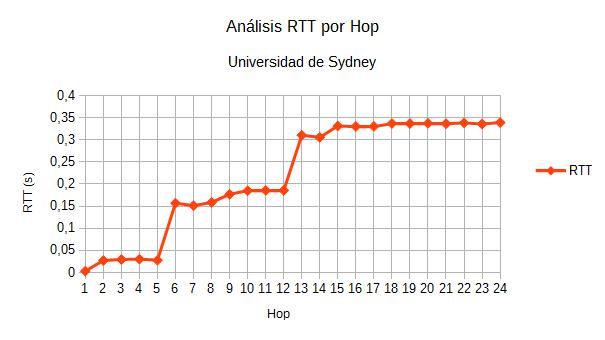
\includegraphics[width=1\textwidth]{graficos/rTT_Australia.jpg}
\caption{RTT promedio por hop - Universidad de Sydney}
\label{Australia_rtt}
\end{figure}

A continuación hemos trazado en un mapa la ruta de nuestro host hasta el host destino ubicado en Australia:
\begin{figure}[H]
\centering
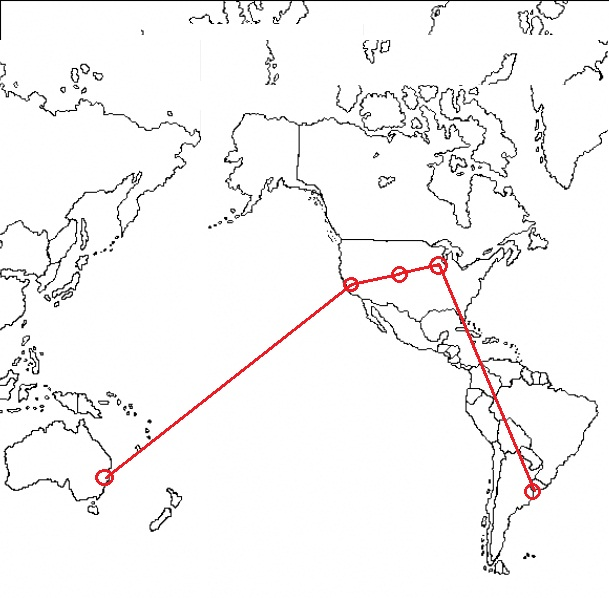
\includegraphics[width=0.8\textwidth]{graficos/mapa_australia.jpg}
\caption{Ruta en Internet - Universidad de Sydney}
\label{australia_zs}
\end{figure}